% ! TeX root = ../../master-thesis.tex

\section{Convergence Simulator}
\label{section:implementation:convergence-simulator}

The implementation of a convergence simulator is described by the class diagram
illustrated in Figure \ref{figure:convergence-simulator-class-diagram}.

\begin{figure}[!ht]
  \centering
  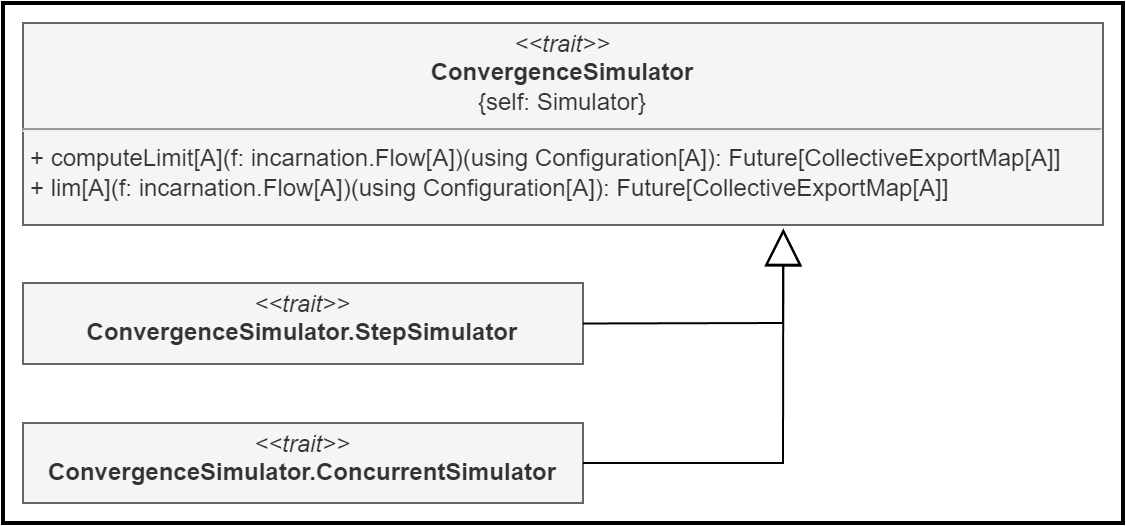
\includegraphics[width=0.60\textwidth]{resources/figures/convergence-simulator-class-diagram.png}
  \caption[A UML class diagram of the convergence simulator]{
    A UML class diagram of the convergence simulator
    and its concrete types.
  }
  \label{figure:convergence-simulator-class-diagram}
\end{figure}

A \texttt{ConvergenceSimulator} is a \texttt{Simulator} with the additional
ability of evaluating the stable state of an aggregate in self-stabilizing
specifications, namely the method \texttt{computeLimit} (or its shorthand
\texttt{lim}). The idea behind \texttt{computeLimit} is as simple as executing
a simulation until its termination, returning the last export transmitted by
each device in the network, in the form of a \texttt{CollectiveExportMap}.
Observation of the environment is possible by leveraging the device sensors
within the specification, attaching their percepts to the device exports.
However, to ensure that the result of \texttt{computeLimit} is a stable state
of the aggregate, the specification should be self-stabilizing and the
simulation should be halted after the aggregate has stabilized. Additionally,
if the aggregate has multiple possible non-deterministic stable states,
\texttt{computeLimit} can only evaluate one of them. Indeed, it may be useful
to consider only the root of the device exports to reduce the number of stable
states of the aggregate, possibly to a single deterministic stable state.

Given a self-stabilizing specification, the result of \texttt{computeLimit} is
determined by the \texttt{HaltPolicy} in the configuration specified by the
user. Below follows an analysis of the suitable \texttt{HaltPolicy}s and their
effects, assuming the user has complete control over the environment:
\begin{itemize}
  \item \texttt{haltWhen(\_ == $N_s$)}: calling $N_s$ the \textit{known} stable
        state of the aggregate, the simulation can be halted when the aggregate
        is in state $N_s$. This policy works for all simulations, however, it
        can only be used for evaluating the \textbf{reachability} of the state
        $N_s$ (\enquote{sometimes $N_s$ holds}), which is a looser property
        compared to convergence (\enquote{sometimes $N_s$ holds forever}).
  \item \texttt{haltAfterDurationOf(T)}: if a stable state exists, after an
        infinite amount of time the aggregate will have certainly stabilized.
        In general, the longer a simulation is executed (i.e., $T$), the
        higher the chances of the aggregate having stabilized. This policy
        works for all simulations, however, relying on real-world time
        introduces non-deterministic results.
  \item \texttt{haltAfterInactivityOf(T)}: inactivity in the simulation can be
        interpreted as a symptom of stability in the aggregate. In general,
        the longer the simulation is inactive (i.e., $T$), the higher the
        chances of the aggregate having stabilized. This policy works the same
        as \texttt{haltAfterDurationOf}, albeit possibly being more flexible
        (e.g., the same value of $T$ may apply to a larger variety of
        simulations).
  \item \texttt{haltAfter(N)}: similar to \texttt{haltAfterDurationOf}, but it
        relies on the steps of a simulation in order to track the simulation
        time. This policy offers deterministic results for deterministic
        simulations, however, it can only be used for \texttt{StepSimulation}s.
  \item \texttt{haltOnVainStep}: this policy guarantees to halt the simulation
        when the aggregate has stabilized, however, it can only be used for
        \texttt{StepSimulation}s.
\end{itemize}

At the moment, two concrete implementations of \texttt{ConvergenceSimulator}
are available, based on the \texttt{StepSimulator} and
\texttt{ConcurrentSimulator}.

\paragraph{Example.}
A practical application of the \texttt{ConvergenceSimulator} is demonstrat\-ed
in the following program (Listing \ref{listing:convergence-simulator-example}).

\lstinputlisting[
  language=Scala,
  caption={
      [An application of the convergence simulator]
      An application of \texttt{ConvergenceSimulator}. The program
      evaluates the stable states for three similar specifications
      (lines 21-23), in which each device counts all the integer numbers in a
      given range. For simplicity, the stable states only show the root of the
      devices exports.
    },
  captionpos=b,
  label={listing:convergence-simulator-example}
]{resources/listings/convergence-simulator-example.txt}
